\subsection{Data}
\label{data_section}
For our experiments, we used three datasets. We will be referring to them as: \dataEN, \dataORG, and \dataDE.
\subsubsection{Amazon EN}
This dataset contains Amazon product reviews and metadata from May 1996 to July 2014. In our case, since we were interested in the organic food domain, we used data from three categories:
\begin{itemize}
  \item Grocery and Gourmet Food
  \item Health and Personal Care
  \item Beauty
\end{itemize}
These three categories contained the following amount of reviews:
\begin{center}
 \begin{tabular}{||c c||} 
 \hline
 Category & Reviews\\ [0.4ex] 
 \hline\hline
 Grocery and Gourmet Food & 198.502\\ 
 \hline
 Health and Personal Care & 151.254\\
 \hline
 Beauty & 346.355\\
 \hline\hline
 Total & 696.111\\
 \hline
\end{tabular}
\end{center}
% As we are interested in the domain of organic food, we filtered all reviews that contained the word "organic". After doing this, we ended up with the following amount of reviews in each category:
Additionally, we filtered all reviews that contained the word "organic". In the end, we ended up with the following amount of reviews in each category:
\begin{center}
 \begin{tabular}{||c c||} 
 \hline
 Category & Reviews\\ [0.4ex] 
 \hline\hline
 Grocery and Gourmet Food & 9.962\\ 
 \hline
 Health and Personal Care & 3.272\\
 \hline
 Beauty & 2.227\\
 \hline\hline
 Total & 15.561 \\
 \hline
\end{tabular}
\end{center}
The percentage distribution of ratings in the dataset is shown in Figure \ref{amazon_en_pie_chart}.\\

\begin{figure}[h]
\centering
\begin{tikzpicture}
    \pie[color={TUMBlau!10, TUMBlau!25, TUMBlau!40, TUMBlau!55, TUMBlau!70},
        radius=1.5,
        text=pin,
        before number=\pgfsetfillopacity{0.0}]
        {4.34/1 (4.34\%), 4.52/2 (4.52\%), 9.87/3 (9.87\%), 19.75/4 (19.75\%), 61.49/5 (61.49\%)}
\end{tikzpicture}
\caption{Percentage distribution of ratings in \dataEN.}
\label{amazon_en_pie_chart}
\end{figure}
We can observe that the dataset is imbalanced. For this reason, we applied a downsampling strategy to balance it for our experiments.\\
To train the MilNets for our experiments, we were interested in getting the individual sentences of each comment. To split the Amazon comments into sentences, we used NLTK, which is a a suite of program modules, covering symbolic and statistical natural language processing \cite{NLTKarticle}.\\
After splitting our comments into sentences, we ended up with {\bf 129.867} sentences. Figure \ref{sentences_per_comment_amazon_en} shows the number of sentences per comment in the dataset.
\begin{figure}[h]
\centerline{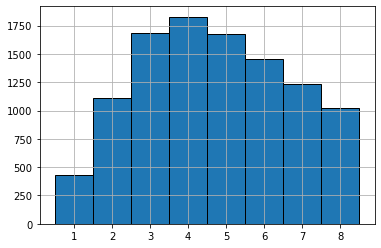
\includegraphics[scale=.4]{images/sentences_per_comment_amazon_en.png}}
\caption{Number of sentences per comment in \dataEN.}
\label{sentences_per_comment_amazon_en}
\end{figure}\\
In this histogram we can see that most of the comments contain between 3 and 5 sentences, which shows that the dataset is appropriate for our MilNet Experiments.\\
In many of our experiments, we used {\bf BERT} to generate embeddings for our sentences. As {\bf BERT} can only handle sentences with a maximum of 512 tokens including [CLS] and [SEP], we removed the outlier sentences that had a large number of tokens. For \dataEN, only 0.2\% of the sentences contain more than 100 tokens. For this reason, we removed all sentences that surpassed that limit.\\
%Figure \ref{amazon_en_tokens_per_sentence} shows the number of tokens per sentence of the dataset after removing the outlier sentences with more than 100 tokens. In this figure we can see that most of the sentences have around 20 tokens.
Figure \ref{amazon_en_tokens_per_sentence} shows the number of tokens per sentence of the dataset after removing the outlier sentences. In this figure we can see that most of the sentences have around 20 tokens.
\begin{figure}[h]
\centerline{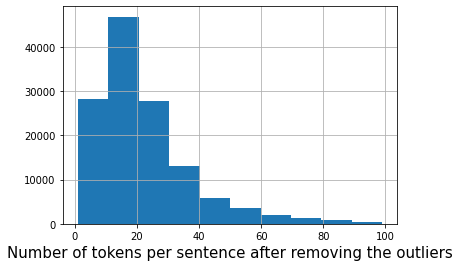
\includegraphics[scale=.5]{images/tokens_per_sentence_amazon_eng_after.png}}
\caption{Number of tokens per sentence in \dataEN.}
\label{amazon_en_tokens_per_sentence}
\end{figure}
\subsubsection{Organic}
This dataset contains sentences with opinions about organic products from Quora. The sentiment of this sentences has been annotated by domain experts with the categories: positive, negative and neutral. The dataset is divided in train, validation and test data.\\
After removing all the 'nan' values, we ended up with the following amount of sentences, with the following distributions:
\begin{center}
 \begin{tabular}{||c c c||} 
 \multicolumn{3}{c}{\bf Train dataset} \\
 \hline
 Sentiment & Sentences & \%\\ [0.4ex] 
 \hline\hline
 positive & 1500 & 32\%\\ 
 \hline
 negative & 1375 & 29.33\%\\
 \hline
 neutral & 1812 & 38.66\\
 \hline\hline
 Total & 4687 & \\
 \hline
\end{tabular}
\end{center}
We can observe that the data is only slightly unbalanced. Therefore, no balancing strategy was applied to this dataset for our experiments.\\
In this dataset, less than 1\% of the data has more than 100 tokens. For this reason, we removed those outliers, just as we did with \dataEN. Figure \ref{organic_tokens_per_sentence} shows the number of tokens per sentence of the dataset after removing the outlier sentences. In this figure we can observe that the final distribution is similar to the one for \dataEN.\\
\begin{figure}[h]
\centerline{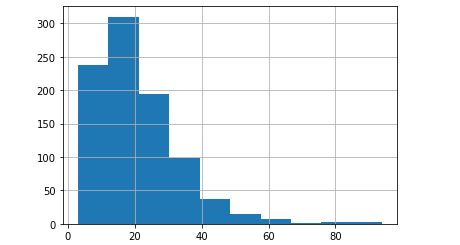
\includegraphics[scale=.5]{images/tokens_per_sentence_organic_after.png}}
\caption{Number of tokens per sentence {\bf Organic}}
\label{organic_tokens_per_sentence}
\end{figure}\\
\subsubsection{Amazon DE}
This dataset contains Amazon reviews in the German language. Since our domain is organic products, we used the data from the two categories:
\begin{itemize}
  \item Grocery
  \item Beauty
\end{itemize}
The dataset contains the following amount of reviews in the selected categories:\\
\begin{center}
 \begin{tabular}{||c c||} 
 \hline
 Category & Reviews\\ [0.4ex] 
 \hline\hline
 Grocery & 2737\\ 
 \hline
 Beauty & 7162\\
 \hline
\end{tabular}
\end{center}
The percentage distribution of ratings in the dataset is shown in Figure \ref{amazon_de_pie_chart}.\\
\begin{figure}[h]
\centering
\begin{tikzpicture}
    \pie[color={TUMBlau!10, TUMBlau!25, TUMBlau!40, TUMBlau!55, TUMBlau!70},
        radius=1.5,
        text=pin,
        before number=\pgfsetfillopacity{0.0}]
        {21.20/1 (21.20\%), 20.63/2 (20.63\%), 20.54/3 (20.54\%),
        18.08/4 (18.08\%), 19.52/5 (19.52\%)}
\end{tikzpicture}
\caption{Percentage distribution of ratings in {\bf amazon DE} dataset.}
\label{amazon_de_pie_chart}
\end{figure}\\
We can observe that the dataset is balanced. For this reason, no balancing strategy was applied to it in our experiments.\\
Just as we did with \dataEN, we used NLTK to split this dataset into sentences. After doing so, we ended up with {\bf 28.994} sentences. Figure \ref{sentences_per_comment_amazon_de} shows the number of sentences per comment in the dataset.\\
\begin{figure}[h]
\centerline{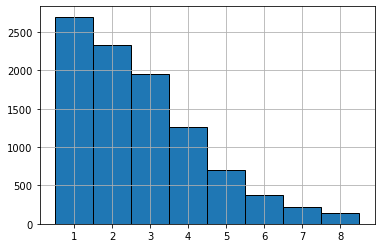
\includegraphics[scale=.5]{images/sentences_per_comment_amazon_de.png}}
\caption{Number of sentences per comment in \dataDE.}
\label{sentences_per_comment_amazon_de}
\end{figure}
After filtering the relevant categories, only 3 sentences in the dataset had more than 100 tokens. We removed these outliers for our experiments. Figure \ref{amazon_de_tokens_per_sentence} shows the number of tokens per sentence after removing the outliers.\\
\begin{figure}[h]
\centerline{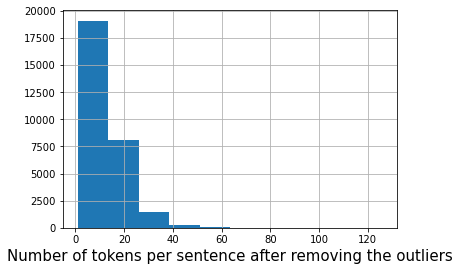
\includegraphics[scale=.5]{images/tokens_per_sentence_amazon_de_after.png}}
\caption{Number of sentences per comment in \dataDE.}
\label{amazon_de_tokens_per_sentence}
\end{figure}
It is interesting to see how different the distributions for \dataDE shown in figure \ref{sentences_per_comment_amazon_de} and figure \ref{amazon_de_tokens_per_sentence} are from those shown in figure \ref{sentences_per_comment_amazon_en} and \ref{amazon_en_tokens_per_sentence} for \dataEN. When comparing these distributions, it can be concluded that German authors tend to write comments with fewer sentences than English ones, but those sentences are longer.
\subsection{Sentiment assessment from review ratings}
In our case, we are interested in using our data to predict sentiment.\\
Given that most of our data consists of Amazon reviews with the number of stars given by the customer, we required a strategy to asses the sentiment of a review based on its stars. The strategy that we used for this purpose is described in Algorithm \ref{sentiment_assesment_algorithm}.\\
\begin{algorithm}[b]
\caption{Sentiment Assessment from number of stars}\label{euclid}
\label{sentiment_assesment_algorithm}
\begin{algorithmic}[1]
\Procedure{SentimentAssessment}{}
\If {$\textit{numberOfStars} < 3$}
    \State $\textit{sentiment} \gets \text{negative}$
\ElsIf {$\textit{numberOfStars} = 3$}
    \State $\textit{sentiment} \gets \text{neutral}$
\Else
    \State $\textit{sentiment} \gets \text{positive}$
\EndIf
\Return \textit{sentiment}
\EndProcedure
\end{algorithmic}
\end{algorithm}
Figure \ref{amazon_sentiment_pie_chart} shows the distribution of sentiment for these datasets after splitting them into sentences and extracting sentiment from them using the described strategy.\\
\begin{figure}[h]
{\bf Amazon EN}:\\
\begin{tikzpicture}
    \pie[color={TUMBlau!10, TUMBlau!40, TUMBlau!70},
        radius=1,
        text=pin,
        before number=\pgfsetfillopacity{0.0}]
        {78.25/positive (78.25\%), 10.63/negative (10.63\%), 11.10/neutral (11.10 \%)}
\end{tikzpicture}\\
{\bf Amazon DE}:\\
\begin{tikzpicture}
       \pie[color={TUMBlau!10, TUMBlau!40, TUMBlau!70},
        radius=1,
        text=pin,
        before number=\pgfsetfillopacity{0.0},
        rotate=90]
        {37.88/positive (37.88\%), 41.84/negative (41.84\%), 20.26/neutral (20.26\%)}
\end{tikzpicture}
\caption{Sentiment distribution for \dataEN and \dataDE after extracting sentiment from reviews}
\label{amazon_sentiment_pie_chart}
\end{figure}\\
In total we had 131.349 sentences in {\dataEN} and 28.994 in {\dataDE}.\\
\subsection{Embeddings}
In our experiments, we used different types of embeddings for our data. In this section we will describe how we got embeddings for each experiment using different models and tools.
\subsubsection{Embeddings for monolingual experiments}
For our monolingual experiments, we used BERT base uncased to generate embeddings for our sentences. For this, we used the tool "Bert as a service".\\
In order to make use of all the syntactic and semantic properties learned by BERT, it is necessary to use a deep layer of the model for the embeddings generation. Nevertheless, the last layer of the model is too close to the target functions, which means that embeddings extracted from this level may be biased towards those targets. For these reasons, we used the second-to-last layer from the BERT model to generate embeddings for the tokens of our sentences.\\
As pooling strategy to get sentence embeddings, we used the mean of the tokens of the sentence.\\
\subsubsection{Embeddings for cross-lingual experiments}
For our cross-lingual experiments, we used different models and tools:\\\\
{\bf Multilingual Bert}:\\
For the cross-lingual BERT experiments, we used the model "Bert Base Multilingual Cased" and the tool "Bert as a service". To generate embeddings for our sentences, we used the -2 layer (second-to-last) and the mean of the tokens as pooling strategy.\\\\
{\bf RoBERTa}:\\
To generate embeddings with RoBERTa, we used the RoBERTa  model provided by the transformers library. Also, we used the library sentence-transformers to generate sentence embeddings. As we did with our other BERT models, we used the -2 layer and the mean of the tokens as pooling strategy.\\\\
{\bf XLING}:\\
For the generation of XLING embeddings, we used the Tensorflow module: universal-sentence-encoder-xling-many. Also, we used the sentencepiece library as tokenizer for our sentences.
\subsubsection{Different context level embeddings}
 \label{contexLeveLEmbeddings}
For the experiment described in section \ref{sentenceCommentLevelContextExperiment}, we used BERT base uncased layer -2 and the mean of the tokens to generate sentence embeddings.
\subsection{Baselines}
In the project, we used different baselines to compare with our results.\\
In this section we are going to explain the baselines we used and the data used for training them.
\subsubsection{Sentiwordnet}
SENTIWORDNET is the result of the automatic annotation of all the synsets of WORDNET according to the notions of “positivity”, “negativity”, and “neutrality”. Each synsets is  associated  to  three numerical  scores: Pos(s), Neg(s), and Obj(s) which  indicate  how  positive, negative, and “objective” (i.e., neutral) the terms contained in the synset are \cite{sentiWordnet}. We used this tool to test sentiment in {\dataEN} and {\dataORG}.\\
Algorithm \ref{sentiwordnet_algorithm_3_classes} shows the prodedure we used to extract sentiment from our sentences using sentiwordnet. In our experiments, we used alpha = 0.3\\
\begin{algorithm}[h]
\caption{Sentiment extraction using Sentiwordnet for three classes}\label{euclid}
\label{sentiwordnet_algorithm_3_classes}
\begin{algorithmic}[1]
\Procedure{GetSentiment (\textit{sentence, alpha})}{}
\For{\textbf{each} word in sentence}
\State $\textit{word} \gets \textit{lemmatizeSentence(word)}$
\State $\textit{word} \gets \textit{getMostCommonSynset(word)}$
\State $\textit{wordSent} \gets \textit{getWordSentiment(word)}$
\State $\textit{sentenceSent} \gets \textit{sentenceSent} + \textit{wordSentPositive} - \textit{wordSentNegative}$
\EndFor
\If {$\textit{alpha} * -1 <= \textit{sentenceSent} <= \textit{alpha}$}
    \Return \textit{neutral}
\ElsIf {$\textit{sentenceSent} >= 0$}
    \Return \textit{positive}
\Else
    \Return \textit{neutral}
\EndIf
\EndProcedure
\end{algorithmic}
\end{algorithm}
For our experiments with two classes, we used the procedure shown in algorithm \ref{sentiwordnet_algorithm_2_classes}.
\begin{algorithm}[h]
\caption{Sentiment extraction using Sentiwordnet for three classes}\label{euclid}
\label{sentiwordnet_algorithm_2_classes}
\begin{algorithmic}[1]
\Procedure{GetSentiment (\textit{sentence, alpha})}{}
\For{\textbf{each} word in sentence}
\State $\textit{word} \gets \textit{lemmatizeSentence(word)}$
\State $\textit{word} \gets \textit{getMostCommonSynset(word)}$
\State $\textit{wordSent} \gets \textit{getWordSentiment(word)}$
\State $\textit{sentenceSent} \gets \textit{sentenceSent} + \textit{wordSentPositive} - \textit{wordSentNegative}$
\EndFor
\If {$\textit{sentenceSent} >= 0$}
    \Return \textit{positive}
\Else
    \Return \textit{negative}
\EndIf
\EndProcedure
\end{algorithmic}
\end{algorithm}
\subsubsection{VADER}
VADER is a simple rule-based model for general sentiment  analysis that performs  exceptionally well  in  the  social  media  domain \cite{VADERarticle}.
In our case, we used VADER to test sentiment in {\dataEN} and {\dataORG}.
\subsubsection{TextBlobDE}
TextBlob is a library for processing textual data. It provides a simple API for diving into common natural language processing tasks such as sentiment analysis \cite{textblob}. TextblobDE is an extension of this library for the German Language. We used TextBlobDE to test sentiment on {\bf Amazon DE}.
\subsubsection{NLTK sentiment analyzer}
For this baseline, we used NLTK Sentiment Analizer to train a Naive Bayes model using our data both for training and testing.
\subsubsection{Scikit-learn SVM model}
As our last baseline, we trained an SVM model using Scikit-learn. For this model, we used bigrams in order to preserve a little bit more context of the sentence for classification.
\subsection{Experiments}
\label{experimentsSection}
For all the experiments, we were using sentence embeddings as input features and comment sentiments as ground truth labels.
\subsubsection{Monolingual analysis}
We started the project with {\it monolingual} experiments --- for this setting, we worked only with data in English, i.e. {\bf amazon EN} and {\bf organic} datasets. \\
The motivation for the whole project was the idea that the {\bf amazon EN} dataset contains some useful information that can help with classifying the {\bf organic} dataset as they share the same domain. Thus, the main experiments for monolingual setting were the following:
\begin{itemize}
    \item {\tt amazon EN-organic} --- training on the {\bf amazon EN} dataset and testing on the {\bf organic} dataset.
    \item {\tt amazon EN-amazon EN} --- training and testing on the {\bf amazon EN} dataset.
\end{itemize}
For both of the experiments, we also had an option of fine-tuning the model on the {\bf organic} dataset. \\
For comparison purposes, we conducted {\tt organic-organic} experiment as well. For this, we considered each sentence in the {\bf organic} dataset as a separate comment, and fed such training data into MilNet. This led to the degenerate attention mechanism in the network as the only attention weight was equal to $1.0$ for every data point. Using this approach, we turned MulNet into a simple RNN model and obtained a competitive baseline for other experiments on the {\bf organic} dataset.

\subsubsection{Cross-lingual analysis}
The next stage of the project was introducing new dataset in German --- {\bf amazon DE}. We were interested how well the model can transfer semantic features from one language to another. Thus, we held out the whole {\bf amazon DE} dataset as a test set and conducted an experiment {\tt amazon EN-amazon DE}. \\
In the cross-lingual setting, we expored different initial embeddings, e.g. BERT multilingual, RoBerta and XLING.
\subsubsection{Different context level embeddings}
\label{sentenceCommentLevelContextExperiment}
Another area of investigation was to see if giving more context to our sentences when generating ist embeddings gave an improvement in the sentiment analysis task.
In our previous experiments, we used only the sentence as context for generating embeddings. For this experiment, we generated the embeddings of our sentences using the entire comment as context.
The following example illustrates this:\\\\
{\bf Generation of sentence-level context embeddings:}\\\\
{\bf Tokenized Comment}: CLS, {\color{TUMBlau}'I', 'really', 'love', 'the', 'product', '.'},{\color{red}'It', 'is', 'really', 'tas', '\#\#ty'}, SEP.\\
\begin{itemize}
  \item Context for the generating embeddings for {\color{TUMBlau} sentence 1}: 'I', 'really', 'love', 'the', 'product', '.'
  \item Tokens used for the generating embeddings for {\color{TUMBlau} sentence 1}: 'I', 'really', 'love', 'the', 'product', '.'
  \item Context for the generating embeddings for {\color{red} sentence 2}: 'It', 'is', 'really', 'tas', '\#\#ty'.
  \item Tokens used for the generating embeddings for {\color{red} sentence 2}: 'It', 'is', 'really', 'tas', '\#\#ty'.
\end{itemize}
{\bf Generation of comment-level context embeddings:}\\\\
{\bf Tokenized Comment}: CLS,{\color{TUMBlau}'I', 'really', 'love', 'the', 'product', '.'},{\color{red}'It', 'is', 'really', 'tas', '\#\#ty'},SEP.
\begin{itemize}
  \item Context for the generating embeddings for {\color{TUMBlau} sentence 1}: 'I', 'really', 'love', 'the', 'product', '.','It', 'is', 'really', 'tas', '\#\#ty'
  \item Tokens used for the generating embeddings for {\color{TUMBlau} sentence 1}: 'I', 'really', 'love', 'the', 'product', '.'
  \item Context for the generating embeddings for {\color{red} sentence 2}: 'I', 'really', 'love', 'the', 'product', '.','It', 'is', 'really', 'tas', '\#\#ty'.
  \item Tokens used for the generating embeddings for {\color{red} sentence 2}: 'It', 'is', 'really', 'tas', '\#\#ty'.
\end{itemize}
For getting both types of embeddings, we used BERT base uncased layer -2 and the mean of the tokens as pooling strategy to get sentences embeddings.\\
As mentioned before, BERT can only handle sentences with a maximum of 512 tokens including [CLS] and [SEP]. In our data, 9,3\% of the comments had 510 tokens or more.\\
After removing these otulier comments, we lost 34\% of our total sentences. This explains why the results in this experiment are lower compared to the other experiments we did.
\subsubsection{Two-class analysis}
The confusion matrix for the conducted experiments gave us a motivation for exploring the reduced problem with only two classes ({\it negative} and {\it positive}). As you can see in Figure \ref{confusion}, {\it neutral} class introduces a lot of confusion for the model. Thus, we dropped the {\it neutral} class from all the datasets and repeated the experiments on this reduced data.
\begin{figure}
\begin{center}
 \begin{tabular}{|c || c | c | c|} 
 \hline
 True & - & 0 & + \\
 \hline
 - & 154 & 67 & 12 \\
 0 & 70 & 174 & 44 \\
 + & 46 & 55 & 141 \\
 \hline
\end{tabular}
\end{center}
\caption{Confusion matrix for {\tt amazon EN-organic} trained on BERT base embeddings.}
\label{confusion}
\end{figure}